\chapter{Исследовательский раздел}

\section{Технические характеристики}

Технические характеристики компьютера, на котором проводился замерный эксперимент:
\begin{itemize}
	\item процессор Intel Core i5-10400F (6 ядер) \cite{intel};
	\item 16 Гб оперативная память DDR4;
	\item операционная система Windows 10 Pro \cite{windows}.
\end{itemize}

Во время проведения исследования ноутбук был нагружен только системными приложениями и целевой программой. 

В библиотеке $time$ языка $python$ есть встроенный функционал для замеров времени.
Для замеров процессорного времени используется функция $process_time$, которая возвращает время в секундах.
Происходит запуск фиксированного числа тестов для каждого случая и вычисляется среднее затраченное время. \cite{python-time}.

\section{Временные показатели}

Обозначения:
\begin{itemize}
	\item матричный Левенштейн (Lev) --- матричная реализация алгоритма поиска расстояния Левенштейна;
	\item матричный ДЛ (Dam-Lev) --- матричная реализация алгоритма поиска расстояния Дамерау-Левенштейна;
	\item рекурсивный ДЛ (Rec) --- рекурсивная реализация алгоритма поиска расстояния Дамерау-Левенштейна;
	\item кэширование ДЛ (Rec-Cache) --- рекурсивная реализация алгоритма поиска расстояния Дамерау-Левенштейна с кэшированием.
\end{itemize}

В таблице \ref{table:time} приведены результаты замеров времени для строк различной длины (в каждом эксперименте длины строк одинаковы) для каждой реализации алгоритмов.

\begin{table}[H]
	\centering
	\footnotesize
	\caption{\label{table:time} Временные замеры различных реализаций поиска редакционных расстояний}
	\begin{center}
		\begin{tabular}{|r|r|r|r|r|}
			\hline
			& \multicolumn{4}{l|}{Время, мс} \\
			\cline{2-5}
			\raisebox{1.5ex}[0cm][0cm]{Длина слова}
			& Матричный Левенштейн & Матричный ДЛ & Рекурсивный ДЛ & Кэширование ДЛ \\
			\hline
			1 & 0.02325 & 0.02375 & 0.0135 & 0.025 \\ \hline
			2 & 0.025 & 0.02625 & 0.0265 & 0.02675 \\ \hline
			3 & 0.0275 & 0.0275 & 0.0645 & 0.0325 \\ \hline
			4 & 0.02875 & 0.03 & 0.15625 & 0.035 \\ \hline
			5 & 0.03125 & 0.03125 & 0.9375 & 0.0425 \\ \hline
			6 & 0.04 & 0.0425 & 3.90625 & 0.0525 \\ \hline
			7 & 0.05025 & 0.055 & 22.03125 & 0.075 \\ \hline
			8 & 0.06775 & 0.0675 & 122.96875 & 0.08225 \\ \hline
			9 & 0.07825 & 0.0925 & 699.21875 & 0.1425 \\ \hline
			10 & 0.16125 & 0.18125 & 3971.5625 & 0.17125 \\ \hline
			20 & 0.3125 & 0.35625 & -- & 0.625 \\ \hline
			40 & 0.78125 & 0.78125 & -- & 1.09375 \\ \hline
			60 & 1.71875 & 2.34375 & -- & 3.125 \\ \hline
			80 & 2.5 & 3.4375 & -- & 5.625 \\ \hline
			100 & 3.59375 & 4.84375 & -- & 9.53125 \\ \hline
			120 & 7.03125 & 7.1875 & -- & 13.4375 \\ \hline
			140 & 7.65625 & 10 & -- & 17.8125 \\ \hline
			160 & 10.78125 & 11.71875 & -- & 22.34375 \\ \hline
			180 & 11.71875 & 15.9375 & -- & 27.96875 \\ \hline
		\end{tabular}
	\end{center}
\end{table}

На рисунке \ref{plt:cpu-matrix} представлен график зависимости процессорного времени от длины слова для матричных реализаций.

На рисунках \ref{plt:cpu-lev}--\ref{plt:cpu-cache} представлены графики зависимости процессорного времени от длины слова.

\begin{figure}[H]
	\centering
	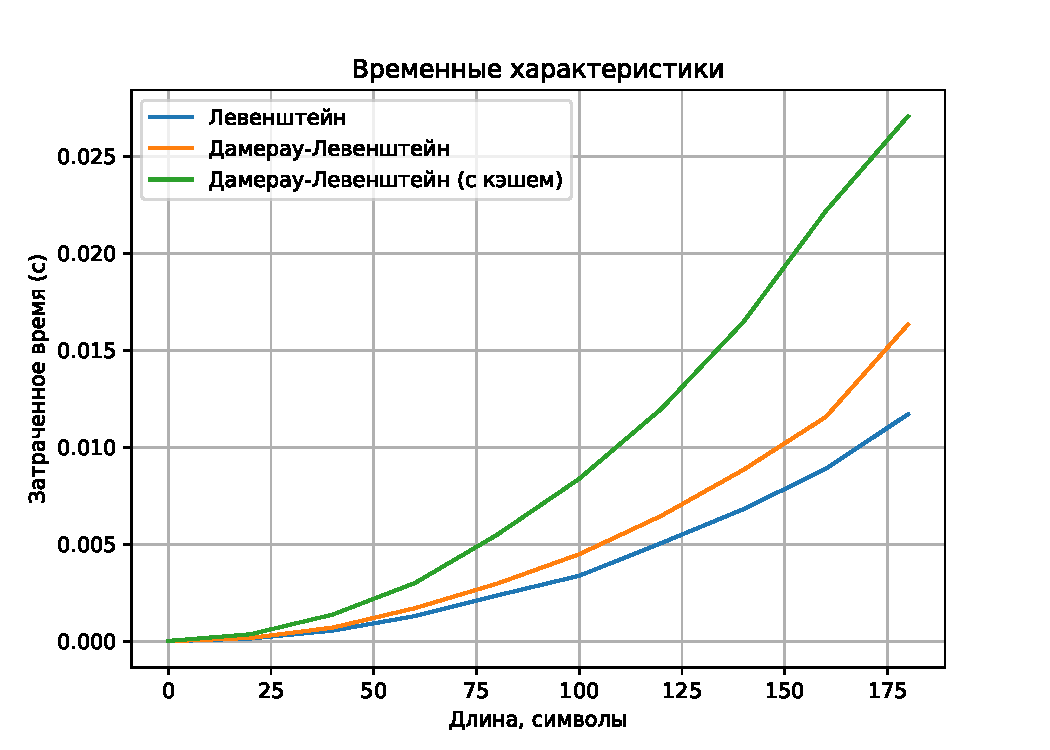
\includegraphics{assets/plots/cpu-matrix.pdf}
	\caption{График зависимости процессорного времени от длины слова}
	\label{plt:cpu-matrix}
\end{figure}

\begin{figure}[H]
	\centering
	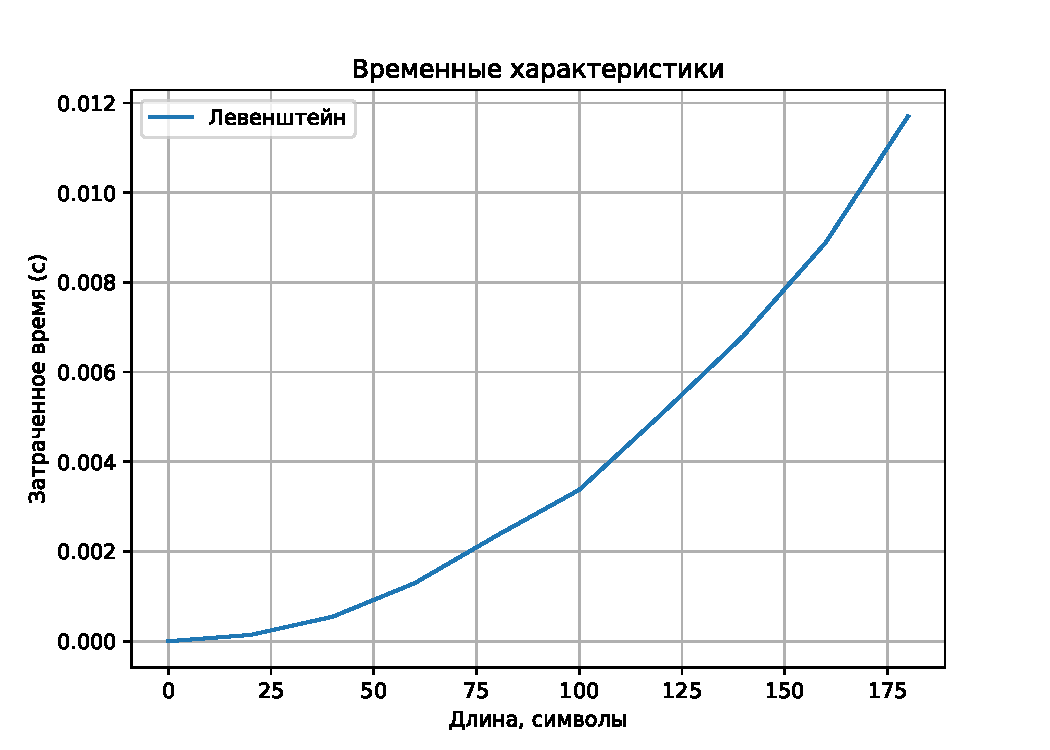
\includegraphics{assets/plots/cpu-lev.pdf}
	\caption{График зависимости процессорного времени от длины слова}
	\label{plt:cpu-lev}
\end{figure}

\begin{figure}[H]
	\centering
	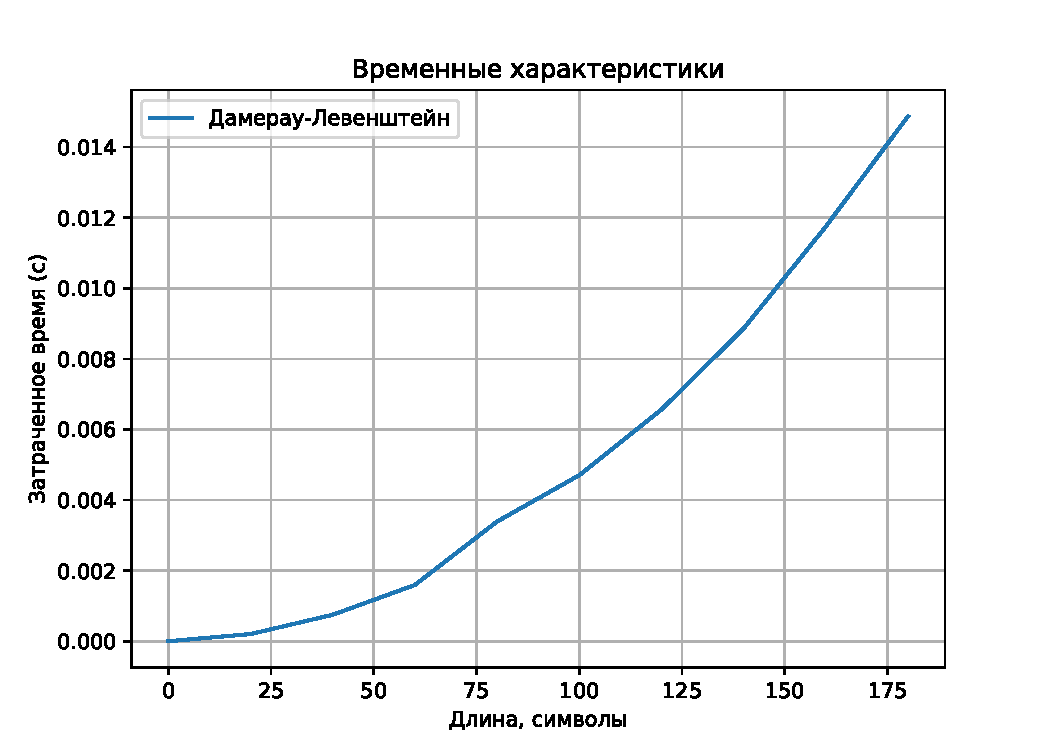
\includegraphics{assets/plots/cpu-dam-lev.pdf}
	\caption{График зависимости процессорного времени от длины слова}
	\label{plt:cpu-dam-lev}
\end{figure}

\begin{figure}[H]
	\centering
	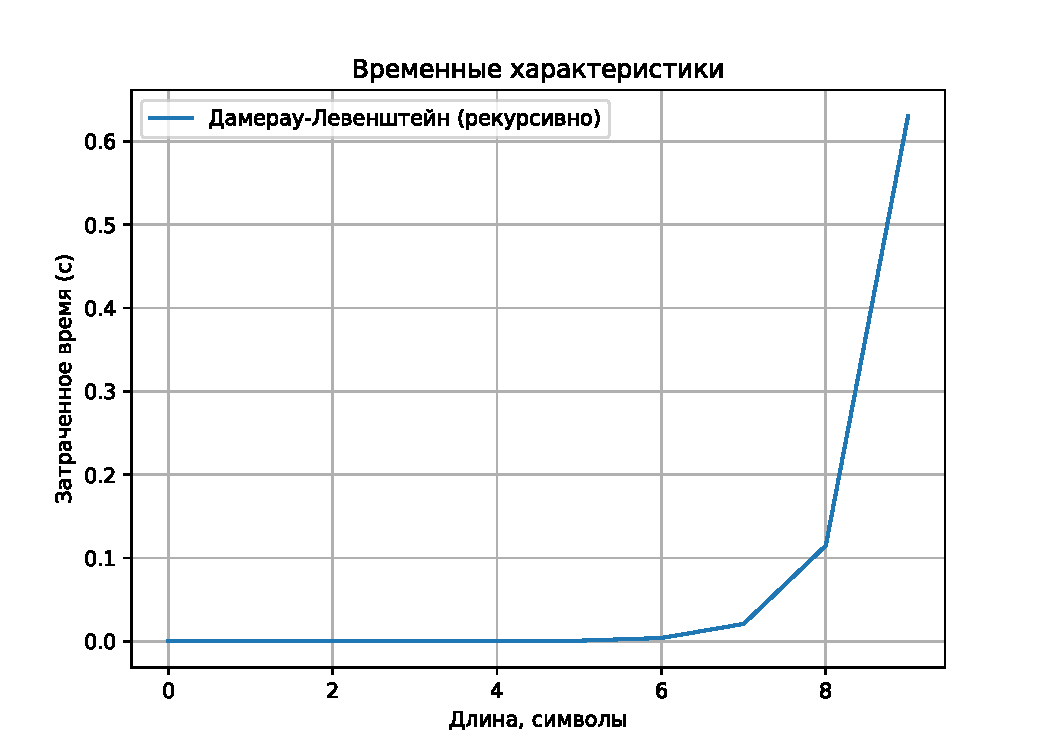
\includegraphics{assets/plots/cpu-rec.pdf}
	\caption{График зависимости процессорного времени от длины слова}
	\label{plt:cpu-rec}
\end{figure}

\begin{figure}[H]
	\centering
	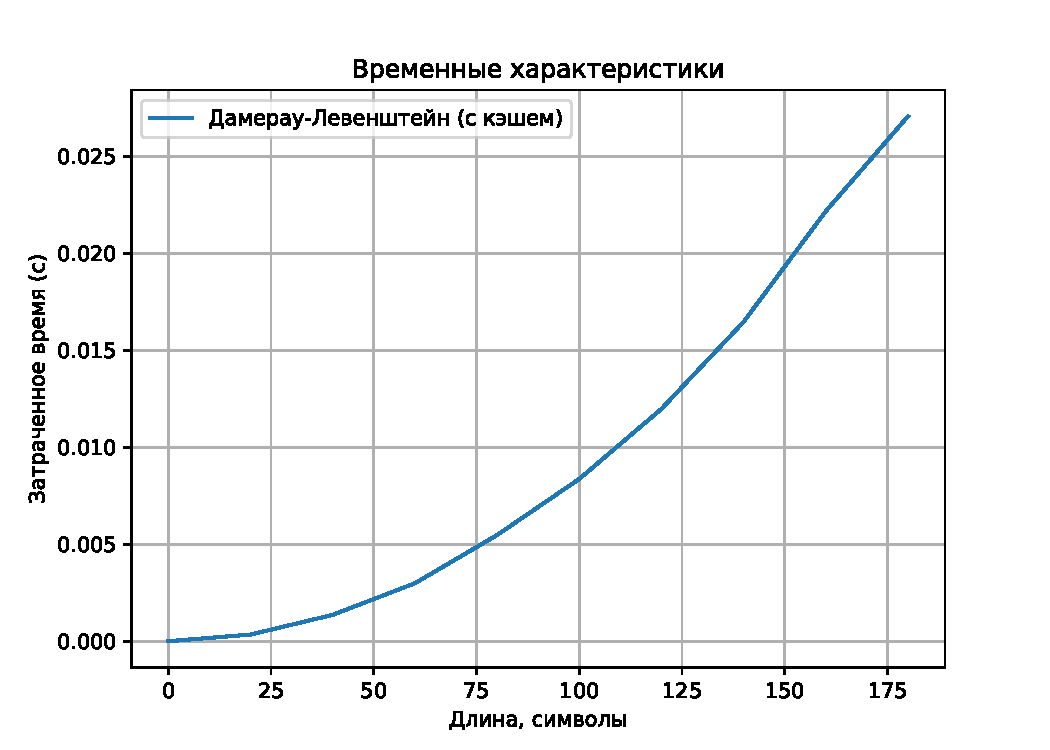
\includegraphics{assets/plots/cpu-cache.pdf}
	\caption{График зависимости процессорного времени от длины слова}
	\label{plt:cpu-cache}
\end{figure}

При длине слова, большей 10, замеры для рекурсивной реализации алгоритма поиска расстояния Дамерау-Левенштейна не производились в связи с заметным отставанием от остальных реализаций.


\section{Теоретические затраты памяти}

Пусть
\begin{itemize}
	\item $len_{1}$ --- длина строки $str_{1}$;
	\item $len_{2}$ --- длина строки $str_{2}$;
	\item $string$ --- массив символьного типа;
	\item $int$ --- целочисленный тип;
	\item $[]int32$ --- массив целочисленного типа;
	\item $[][]int32$ --- матрица целочисленного типа;
	\item $size()$ --- функция, вычисляющая размер в байтах.
\end{itemize}

Использование памяти при итеративной реализации алгоритма поиска расстояния Левенштейна теоретически равно:
\begin{equation}
	\begin{aligned}
		(len_{1} + 1) \cdot (len_{2} + 1) \cdot size(int32) + 2 \cdot size(string) + 5 \cdot size(int32),
	\end{aligned}
\end{equation}
где 
\begin{itemize}
	\item $2 \cdot size(string)$ --- хранение двух строк;
	\item $5 \cdot size(int32)$ --- хранение размеров матрицы, адреса возврата и дополнительная переменная для хранения результата.
\end{itemize}

Использование памяти при итеративной реализации алгоритма поиска расстояния Дамерау---Левенштейна теоретически равно:
\begin{equation}
	\begin{aligned}
		(len_{1} + 1) \cdot (len_{2} + 1) \cdot size(int) + 2 \cdot size(string) + 5 \cdot size(int32),
	\end{aligned}
\end{equation}
где 
\begin{itemize}
	\item $2 \cdot size(string)$ --- хранение двух строк;
	\item $5 \cdot size(int32)$ --- хранение размеров матрицы, адреса возврата и дополнительная переменная для хранения результата.
\end{itemize}

Так как при каждом вызове в рекурсивном алгоритме нахождения расстояния Дамерау---Левенштейна требуется 2 дополнительные переменные и, при этом, максимальная глубина стека вызовов равна сумме длин входящих строк, то в худшем случае расход памяти равен:
\begin{equation}
	(len_{1} + len_{2}) \cdot (2 \cdot size(string) + 5 \cdot size(int32)),
\end{equation}
где:
\begin{itemize}
	\item $2 \cdot size(string)$ --- хранение двух строк;
	\item $5 \cdot size(int32)$ --- дополнительные переменные, адрес возврата и длины строк.
\end{itemize}

В случае использования рекурсивного алгоритма поиска расстояния Дамерау---Левенштейна с кэшированием необходимо так же учитывать размеры матрицы, поэтому в худшем случае расход памяти равен:
\begin{equation}
	\begin{aligned}
		(len_{1} + len_{2}) \cdot (2 \cdot size(string) + 5 \cdot size(int32) + \\ + (len_{1} + 1) \cdot (len_{2} + 1) \cdot size(int32))
	\end{aligned}
\end{equation}

\section*{Вывод} \addcontentsline{toc}{section}{\numberline {}}

В этом разделе было осуществлено сравнение различных алгоритмов, решающих проблему поиска расстояний Левенштейна и Дамерау---Левенштейна по затрачиваемой памяти и процессорному времени. 
Самыми быстрыми алгоритмами с равными затратами памяти можно считать матричные реализации алгоритма нахождения расстояний Левенштейна и Дамерау---Левенштейна.
Рекурсивная реализация алгоритма нахождения расстояния Дамерау---Левенштейна с кэшированием проигрывает матричным реализациям в 1.5-2 раза при одинаковых затратах памяти. 
Рекурсивная реализация алгоритма нахождения расстояния Дамерау-Левенштейна многократно выигрывает все остальные реализации по затратам памяти, однако многократно проигрывает по затратам процессорного времени при любой длине слова.